\section{Existing approaches in influenza computational modelling}

Seasonal and zoonotic influenza is a popular subject of viral modelling, which has a variety of approaches. The majority of viral models use systems of ordinary differential equations (ODE), but partial (PDE) and delay differential equations (DDE) have also been implemented.

\begin{figure}
\begin{center}
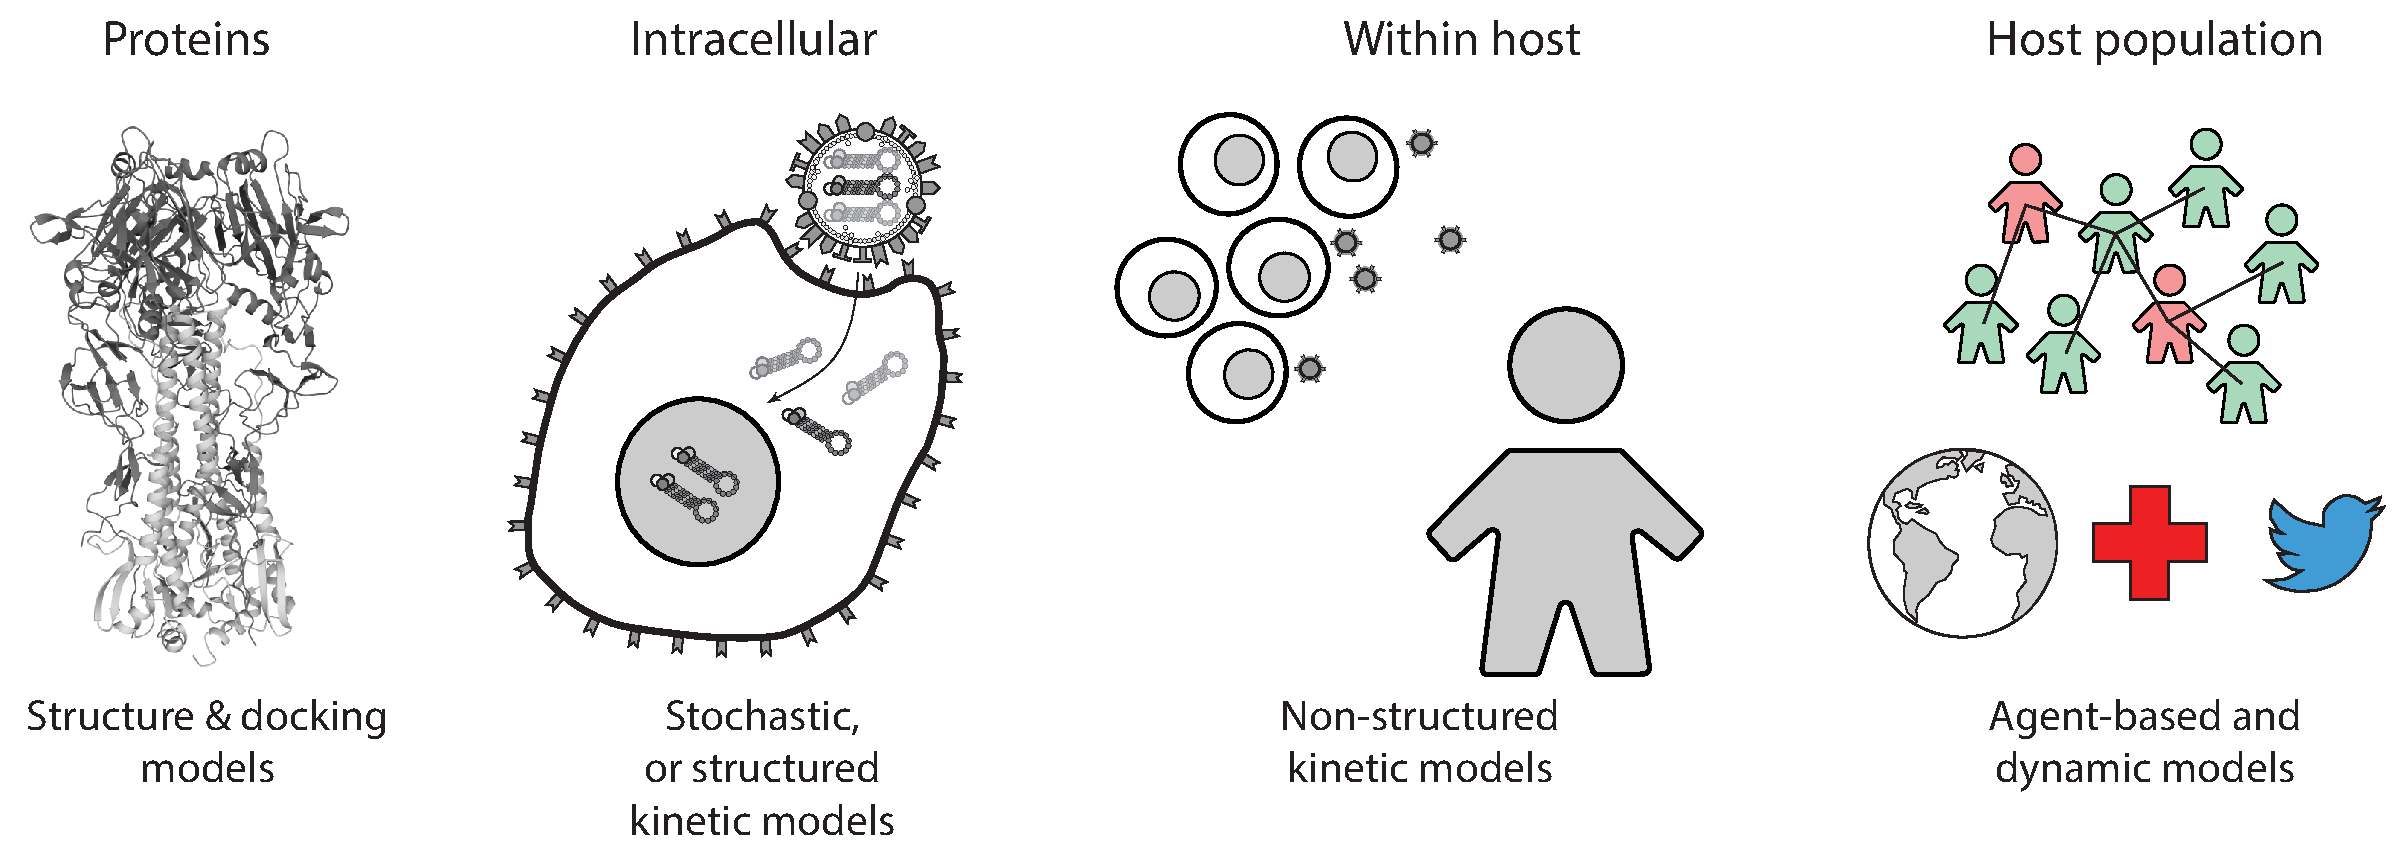
\includegraphics[width=1\textwidth, trim={0cm 0cm 0cm 0cm}, clip]{D_chapters/0_introduction/viralModelling copy.pdf}
\caption[Influenza computational modelling approaches on different scales]{Influenza computational modelling approaches on different scales. \par Hemagglutinin protein structure is a black and white render from \cite{influenzaVirusHemagglutininPDB}.}
\label{figure:modellingApproachesInfluenza}
\end{center}
\end{figure}

The knowledge of amino acid sequence and protein folding allow to predict the structure \cite{lin2007structure, russell2018influenza} of the viral proteins, and how they can bind to their targets or inhibitors \cite{li2015inhibitors, jagadesh2016influenza}.

On intracellular level, stochastic and structured kinetic approaches are used to model specific processes during the infection. Structured models which include individual processes in virus replication \cite{sidorenko2004structured}, endosomal escape \cite{lagache2012modeling} and defective viral particle propagation \cite{rudiger2019multiscale} have been proposed. Their phenomenological nature means that they often rely on unobserved quantities and variables, and do not allow for inference on specific molecular targets for intervention.

Non-structured kinetic models are used to describe the transmission within the host – cell culture or an individual. These models aim to understand and quantify the progression of the infection, and determine its resulting severity and duration \cite{beauchemin2008modeling}. We further discuss existing non-structured kinetic models and their applications in Chapter \ref{ch:DARPin}.

Finally, to describe the transmission between the hosts, people use dynamic or agent-based models. Influenza infection dynamic models are focused primarily capturing the transmission between hosts, with the goal of informing public health decisions and assist in pandemic planning \cite{ferguson2006strategies, mcvernon2007model}. With the advancement of social media, a new type of influenza forecasting models has emerged \cite{pawelek2014modeling, santillana2015combining, levy2018modeling}, relying on publicly available self-reporting by users. Agent-based models incorporate individual behavioral patterns to determine how social policies and educational efforts can affect viral spread within the population \cite{karimi2015effect}.

Despite the abundance of knowledge about influenza and its components, these approaches are used separately, and rarely make use of knowledge obtained through other methods, which makes mechanistic predictions about the underlying processes difficult. The reason for this is that combining these various levels of description in a meaningful manner is a non-trivial problem.
